\documentclass[10pt,a4paper]{article}
\usepackage[margin=19mm]{geometry}
\usepackage[T1]{fontenc}
\usepackage{lmodern}
\usepackage{amsmath,amssymb,booktabs,longtable,array,enumitem,listings}
\usepackage{tikz}
\usetikzlibrary{arrows.meta,positioning,fit}
\usepackage[hidelinks]{hyperref}
\setlist{nosep,leftmargin=*}
\setlength{\emergencystretch}{3em}
\newcommand{\code}[1]{{\small\nolinkurl{#1}}}
\setlength{\tabcolsep}{2pt}
\newcolumntype{L}[1]{>{\raggedright\arraybackslash}p{#1}}
\lstset{basicstyle=\ttfamily\small,breaklines=true,columns=fullflexible,keepspaces=true,frame=single}
\title{Canonical cell storage and borrowed mathematical views\\Repository-grounded API and migration plan}
\author{HyMeKo Core / Graph / runtime integration}
\date{Created-at: 2026-09-21 15:10 +02:00}
\begin{document}
\maketitle
\noindent\textbf{PlanOnly.} No architecture refactor, protected source edit, manifest/lockfile change, commit, push, or benchmark campaign is performed by this task. Current-task \code{CORE.YAML} items touched: \textbf{empty}.

\medskip
\noindent\textbf{Recommendation.} Introduce a move-only storage ownership boundary inside the existing \code{PreparedIr}; keep the existing \code{Ir} compatibility representation and \code{IncidenceView}. Extend Graph's existing matroid infrastructure later. Separate search rollback from physical graph editing.

\medskip
\noindent\textbf{Estimates, not measurements.} Plan artifact completion: approximately 15--20 minutes after creation for writing, two PDF passes, inspection and archival. First implementation slice: approximately 3--5 engineering hours after authorization: small owner module, private owner substitution, regression/allocation checks, downstream checks and report. Later phases need estimates after their decision gates; no complete-machine or MCU delivery date is promised.

\medskip
\noindent\textbf{Scope.} Preserve the canonical IR and web, desktop and XR integrations while defining neutral storage, mathematical projections, versioned validity, reversible search and eventual bounded structural operations. First slice needs no new dependency. Proposed APIs are design contracts, not existing code.
\tableofcontents
\newpage

\section{Checkout and dependency baseline}
\label{sec:baseline}
Paths are relative to the named checkout; most are siblings under \code{D:/hakiko_ai_ws/03_implementation/hymeko_framework}. Discovery combines manifests, source bodies, tests, reports and actual call chains. Searches locate code; they do not prove behavior.
\begin{longtable}{L{25mm}L{57mm}L{21mm}L{63mm}}
\toprule Checkout & Branch & HEAD & State\\\midrule
Core & feat/ir-runtime-updates & 10138bfc14fc & Refreshed, upstream 0/0; three pre-existing untracked TeX byproducts.\\
Web & feat/scenario-runtime & 68955a16bbf9 & Clean; handoff commit one ahead of upstream.\\
Graph & chore/published-ir-runtime & be8da9cfe41c & Refreshed, upstream 0/0; existing untracked reports/TeX byproducts.\\
Parser & master & be52aac1270f & Clean; consumers resolve pinned f11628591a81.\\
Transformation & feat/robotics-authoring-integration & a0b5420f2420 & Existing geometry/query, docs, manifest/lock changes preserved.\\
Kawamirai & feat/xr-passthrough-rendering & 050991eca880 & Existing Cargo manifest/lock changes.\\
XR & feat/native-quest-workbench & d674d722172a & Existing native/Quest/editor changes; locked resolution fails.\\
Simulator XR publish & feat/quest-immersive-ui & 4da272914598 & Existing dirty worktree outside framework preserved.\\
Tensor & main & 5ab2c33b6d3c & Refreshed, clean, upstream 0/0.\\
Hotaru & main & 5787b0c25e16 & Refreshed, clean, upstream 0/0.\\
Hive & feat/lan-model-catalog & e708ff6f1e3e & Refreshed, clean, upstream 0/0.\\
Akoire & feat/belief-planner & 2e64c4bf3d2d & Refreshed, clean, upstream 0/0.\\
Robotics & feat/robotics-belief-planner & 9ec076c629cb & Refreshed, upstream 0/0; existing README/docs changes.\\
RL & main & a008b7e473ea & Refreshed, clean, upstream 0/0.\\
Nagare & fix/local-tensor-paths & 8732738e931c & Outside framework; read-only audit, not refreshed/rebuilt here.\\
\bottomrule
\end{longtable}
The initial workspace provider outside framework is \code{4aa27f2}, eight behind refreshed origin/main. Core imports a different sibling provider under framework: \code{e3cea77fa1bb}, branch \code{docs/hymeko-authoring-principles}. Nagare's entry point requests a provider revision different from its actual sibling; reconcile activation before future Nagare implementation/validation. No checkout was cleaned, worktree created or branch switched.

\paragraph{Resolved versus declared dependencies.}
Core's locked offline dependency tree succeeded. Web's existing \code{scripts/build.mjs} wrapper, with existing local cargo config and XR/Kawamirai path settings, resolved native and wasm trees successfully with one Core and Parser package identity on those checked paths. This is local integration, not a demonstrated portable release. Web declares Core \code{2c4e07244de5}; the local patch supplies \code{10138bfc14fc}. Parser HEAD is not the consumed revision. Transformation geometry/query are path-patched while other consumers can resolve published code; Tensor's published pin also differs from checkout HEAD.

\code{npm ls --depth=0 --offline} passed. Rust/Cargo 1.97.1, Node 26.8.1, native Windows, wasm32 and aarch64 Android targets were available. XR's locked tree failed because current manifests require a lockfile update; its dirty lockfile was not rewritten. Native Quest integration is an unresolved gate. Dependency discovery does not replace runtime tests.

\paragraph{Evidence limits.}
Web's September 21 handoff remains the client starting point. Registry/older platform prose has drift: Web is absent from the registry, HNN ownership predates relocation to Nagare, and old CBOR policy predates the current checked snapshot codec. Actual code, handoff and canonical roadmap phase order must be reconciled explicitly.

Relevant existing plans: August 30 dense-view/index boundary; August 31 generational arenas; September 1 incidence navigation; September 15 snapshot/CBOR stream installation; September 17 semantic reads. This new ownership/projection plan does not replace those distinct scopes.

\section{Current architecture, symbols and call chains}
\label{sec:architecture}
\begin{center}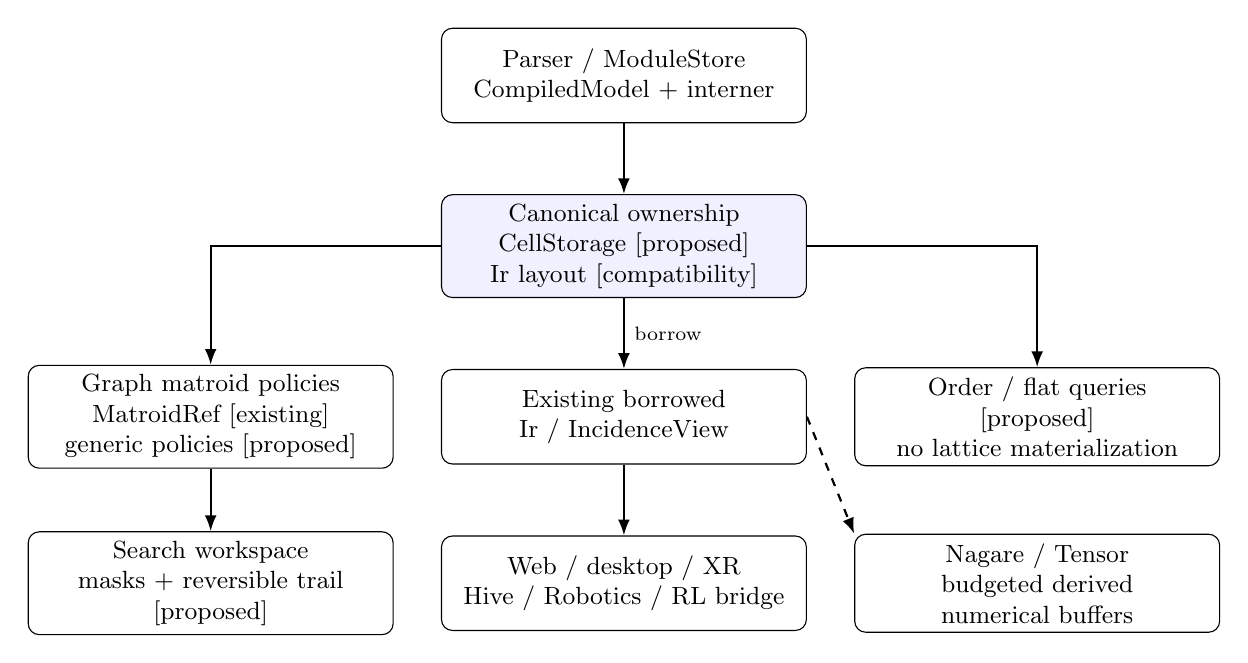
\begin{tikzpicture}[
 box/.style={draw,rounded corners,align=center,font=\small,text width=44mm,minimum height=12mm},
 arrow/.style={-{Latex[length=2mm]},thick},node distance=9mm and 6mm]
\node[box] (source) {Parser / ModuleStore\\CompiledModel + interner};
\node[box,below=of source,fill=blue!6] (storage) {Canonical ownership\\CellStorage [proposed]\\Ir layout [compatibility]};
\node[box,below=of storage] (hyper) {Existing borrowed\\Ir / IncidenceView};
\node[box,left=of hyper] (matroid) {Graph matroid policies\\MatroidRef [existing]\\generic policies [proposed]};
\node[box,right=of hyper] (flat) {Order / flat queries\\{[proposed]}\\no lattice materialization};
\node[box,below=of hyper] (clients) {Web / desktop / XR\\Hive / Robotics / RL bridge};
\node[box,left=of clients] (search) {Search workspace\\masks + reversible trail\\{[proposed]}};
\node[box,right=of clients] (compute) {Nagare / Tensor\\budgeted derived\\numerical buffers};
\draw[arrow] (source) -- (storage);
\draw[arrow] (storage) -- node[right,font=\scriptsize]{borrow} (hyper);
\draw[arrow] (storage.west) -| (matroid.north);
\draw[arrow] (storage.east) -| (flat.north);
\draw[arrow] (hyper) -- (clients);
\draw[arrow] (matroid) -- (search);
\draw[arrow,dashed] (hyper.east) -- (compute.north west);
\end{tikzpicture}
\end{center}
\begin{longtable}{L{37mm}L{129mm}}
\toprule Owner/symbol & Observed behavior\\\midrule
Core \code{ir/ir.rs::Ir} & Owns declarations, nodes, edges, arcs, file provenance, namespace roots, annotations, optional model facets, hashes and metadata. Authoritative semantic IR, not generic cell storage. Public vectors permit direct writes.\\
\code{DeclNode}, \code{DeclKind} & Node/Edge/HyperArc declaration kind; parent/child/sibling hierarchy. Typed declarations and record dispatch must remain coherent.\\
\code{NodeRec}, \code{EdgeRec}, \code{ArcRec} & Node/edge bases; ordered edge arc handles; arc owning edge declaration and ordered signed references. Anonymous arcs need not have named declarations.\\
\code{RefAtomR}, \code{SignedRefR} & Target, annotations, optional weights and PortDirection. Plus/Minus/Neutral sign is orthogonal to In/Out/Unspecified direction. Repeated references and slots are semantic.\\
\code{common/ids.rs::Id<Tag>} & Typed usize with phantom tag, public new/raw and NONE sentinel; no owner, generation or foreign-handle detection from numeric value alone.\\
\code{ir/access.rs} & Existing storage-oriented record lookup/coherence accessors; reuse rather than duplicating getters.\\
\code{IncidenceIndexData} & Derived row offsets, arc IDs and slots: retained O(D+I), not a constant-sized cache. Exact-bijection validation needs work/scratch. No copied semantic incidence payload.\\
\code{IncidenceIndex<'ir>} & Borrows Ir, owns derived arrays.\\
\code{PreparedIr}, \code{IncidenceView} & Owned Ir plus lifetime-free index data; two-reference Copy view constructed O(1), zero allocation. Safe borrows prevent mutation while views exist.\\
\code{IncidenceOperatorPlan} & O(I) derived coefficients can depend on values/weights as well as topology.\\
\code{CompiledProgram}, \code{CompiledModel} & Program owns root/index/Ir/imports/hash; model couples shared program and interner.\\
\code{ExecutionState} & RwLock-protected Arc snapshots; prepare/commit owner and base checks; atomic whole-model publication.\\
Graph \code{MatroidRef} & Existing one-word borrowed IncidenceIndex facade; zero-allocation tests and graphic/incremental algorithms.\\
P-graph \code{PGraphView} & Borrowed index and domain classification sets; no copied topology in view. LoweredPGraph/schema still materialize domain topology elsewhere.\\
Nagare \code{HyperGraphView} & Owned dense mappings and incidence arrays in both orientations; derived compute data, not zero-copy structural view.\\
\bottomrule
\end{longtable}

\begin{enumerate}
\item Core \code{module_store/module_store.rs::ModuleStore::compile}: load, real parser, intern/link, build/resolve symbol index, lower, evaluate constants/hash. Linking can clone imported syntax. Root cache belongs to a store; \code{CompiledModel::compile} creates a fresh store.
\item \code{module_store/execution.rs}: model retains program/interner; prepare compiles outside publication lock, commit checks owner and captured base Arc identity. Old readers retain coherent old snapshots.
\item \code{module_store/execution/value_updates.rs::with_value_updates}: validate supported leaf updates, clone Ir/interner/index, preserve IDs/topology, invalidate hash data, validate result. Arbitrary dependent expressions are not reevaluated. Cost is model-sized, not O(delta).
\item \code{writers/cbor_writer.rs::encode_compiled}: delegates to encode, which currently clones Ir/index/string payloads. Decode performs bounded validation into private \code{DecodedCborPayload}; \code{CompiledModel::from_decoded_cbor} installs without reparsing. \code{writers/cbor_writer/stream.rs} bridges to ir\_stream begin/chunk/commit; assembler stages transport bytes, not structural commands.
\item Web \code{crates/hymeko_wasm/src/document.rs::Document::compile_files}: ModuleStore compilation, source span mapping, incidence index in owner/dependent bundle. Reachability and shortest path use Graph on that backing. DocumentView borrows Ir but owns a string-table copy; queries can allocate path indexes/results.
\item Web \code{crates/hymeko_editor/src/session.rs}: source undo/edit history and recompilation. Native XR uses CompiledModel value updates; Quest uses shared Document/Inspector interfaces. Layout/drag data is presentation, not structural authority.
\item Hive \code{src/lib.rs::IrSession}: ExecutionState replace/patch via checked model preparation/commit. Robotics uses borrowed Ir/shared models and publishes recording updates through ExecutionState. Akoire composes domain planning results; no generic cell search found in scoped audit.
\item Nagare \code{src/hnn/traversal/hypergraphview.rs::try_from_ir}: validate and materialize dense compute arrays; edge-target refs excluded by vertex-centric policy. \code{src/runtime.rs::NagareRuntime} predicts/trains numerical graph inputs, not cell instructions.
\item RL \code{hymeko_rl/coin_delivery/cip/hymeko_model.py::emit_control_records}: \code{_run_transform("cip_control", ...)} through framework CLI, parse records, schema-v0 external ControlModel validation. Serialized domain bridge, not a borrowed Rust view. No training is needed here.
\end{enumerate}

\paragraph{Existing matroids and search.}
Graph \code{hymeko_graph/src/matroid/{facade,rank2,levi,workspace}.rs} is the extension owner. Rank2 means arity-two graphic edges, not matroid rank at most two. Parallel arcs stay distinct. Levi elements are \code{(HyperArcId, slot)} with node-plus-arc endpoints; repeated slots are distinct edges, non-node targets typed errors. Forgetting signs/directions is specific to connectivity projection.

Hotaru's \code{src/hypergraph} also contains owned CSR-style algorithm representations; these are not an alternative canonical IR and are not automatically zero-copy. Tensor's numerical rank-like diagnostics (for example stable-rank proxies) are not matroid rank. No general independence-oracle/uniform/GF(2) matroid implementation was found in the scoped source searches; existing graphic policies should be extended first.

GraphicMatroidWorkspace uses DSU arrays and lazy generations. Find performs path-halving writes; incremental sessions have no rollback. Journal every such write or use a reversible non-compressing mode in that owner. Undoing only successful unions is wrong.

P-graph \code{hymeko_pgraph/src/abb.rs::solve_with_regime} recursively includes/excludes units over one shared problem, but clones optimistic BTreeSets and incumbents. Floating subtraction does not ensure bit-exact cost undo. This is minimization: do not silently reuse its pruning orientation for maximization. Generic mathematics belongs in Graph; domain ABB remains P-graph-owned; optimization lowering/backends remain \code{hymeko_optimize}-owned.

\section{Gaps and design choices}
\label{sec:gaps}
Ir already supplies canonical authority but fixes hypergraph/semantic layout and exposes structural vectors. Current handles and constructors are append-oriented, not checked edit sessions. Borrowed views assume frozen backing. Generic matroid policy, canonical structural rollback and explicit order queries are absent. Some compute/client paths deliberately allocate derived data. MCU/HSM execution is a target, not current semantics.

Start with immutable ownership, then checked provenance/projections, then owner adoption and neutral private records. Keep existing mathematical views and budget large derived workspaces explicitly. Do not promise allocation-free queries, serializers or model publication.

Rejected first steps: a CellStorage type alias creates no boundary; a second graph converter duplicates authority; wholesale vector replacement is too broad; a duplicate HypergraphView merely renames existing access/incidence APIs. Wrapping Ir is deliberately transitional, not proof that the physical layout is already mathematically neutral.

\section{Minimal formal model and operational algebra}
\label{sec:formal}
\subsection{Destination, independent of initial layout}
A state has finite live opaque cell identities, typed ordered relation occurrences, payloads and interpretation/provenance facets. Write $C=(H,R,P,F)$ as notation, not an array-of-objects mandate. Relations distinguish containment, bases, incidence and value references; each occurrence records owner, occurrence identity, target, category and attributes. Hypergraph Node/Edge/HyperArc roles are compatibility facets, not intrinsic generic cell types.

Storage consistency checks endpoints/ranges/internal references. Hypergraph validity and matroid axioms are separate predicates. Migration must preserve anonymous arcs, legal unbound declarations, repeated equal-target incidences, arc ordering, signed/weighted bases, hierarchy, symbol/interner pairing, files and model facets. Occurrence identity differs from target identity.

\subsection{Logical versus physical mutation}
Proposed command vocabulary, adapted later to validated existing primitives:
\begin{itemize}
\item \code{CreateCell(temp, facet, payload)} introduces a batch-local identity; physical handles follow transaction policy.
\item \code{DeleteCell(handle, policy)} initially rejects incoming references; no implicit recursive cascade.
\item \code{Attach(owner, relation, occurrence, target, attributes)} preserves ordered placement, multiplicity, sign, direction and roles.
\item \code{Detach(owner, occurrence)} removes exactly one occurrence; target-only removal is ambiguous.
\item Supported payload edits reuse established checked value-update semantics, not disguised topology operations.
\end{itemize}
Existing \code{Ir::push_decl} appends. \code{bind_node_decl}, \code{bind_edge_decl}, \code{bind_arc_decl} bind declaration dispatch, not incidence. Their private path uses index access/debug assertions; it is not a complete externally checked transaction API. No general deletion/unbind was found.

Let $A^*$ be finite command sequences. Concatenation and empty sequence form a free monoid. Each command denotes a partial transformation, with $T_\epsilon(c)=c$ and $T_{uv}(c)=T_v(T_u(c))$ only when intermediate state/preconditions exist. Remove is not universally inverse to add; invalid operations, resource exhaustion and escaped handles remain observable.

Normalization permits only proved rewrites: coalesce payload writes without intervening reads; commute disjoint read/write dependencies; cancel create/delete only without escaping handles, dependent relations or changed error/budget/log semantics. Validate the logical sequence before eliminating actions that could hide errors. Account separately for submitted commands, normalized commands, validation work and physical writes. No normalization engine in slice one.

\subsection{Identity, deletion and rollback}
Keep current IDs/wire encoding initially. Future editable generations begin with no slot reuse; deletion requires explicit liveness/tombstones or indirection. External batches capture source provenance because numeric IDs alone cannot identify foreign handles. Generation-tagged reuse is a later measured choice.

Old published snapshots remain readable. Exclusive structural edits require a unique borrow and released views. Concurrent readers plus incremental edits may motivate paged copy-on-write or a bounded overlay with one authoritative resolution rule; measure their costs before choosing. Compaction needs an explicit remapping boundary, never silent invalidation.

Rollback records old bits, lengths, dispatch/hierarchy/liveness and affected derived state. Restore floats from saved values, not arithmetic inverse. Exact canonical/cache/version restoration differs from allocator-state restoration: retained capacity/high-water allocation may remain unless explicitly prohibited.

\section{Interfaces, ownership and zero-copy}
\label{sec:api}
\subsection{Exact first-slice API}
One new owner retains the current private Ir layout:
\begin{lstlisting}
// Proposed core::ir::storage API; not implemented
pub struct CellStorage { ir: Ir }
impl CellStorage {
    pub fn from_ir(ir: Ir) -> Self;
    pub fn ir(&self) -> &Ir;
    pub fn into_ir(self) -> Ir;
}
// Existing PreparedIr private fields become:
// { storage: CellStorage, data: IncidenceIndexData }
impl PreparedIr {
    pub fn new(ir: Ir) -> Result<Self, IncidenceError>; // unchanged
    pub fn from_storage(storage: CellStorage)
        -> Result<Self, IncidenceError>;              // additive
    pub fn storage(&self) -> &CellStorage;            // additive
    pub fn ir(&self) -> &Ir;                          // unchanged
    pub fn index(&self) -> &IncidenceIndexData;       // unchanged
    pub fn incidences(&self) -> IncidenceView<'_, '_>;// unchanged
    pub fn star_operator(&self) -> StarOperator<'_, '_>;
    pub fn into_ir(self) -> Ir;                       // unchanged
}
\end{lstlisting}
\code{from_ir} moves without allocation/clone; it does not certify arbitrary Ir validity. \code{from_storage} builds/validates the existing index with the same errors; \code{new} delegates to this single path. \code{ir} borrows the stored object; \code{into_ir} consumes it. No Clone, DerefMut, interior mutation, serde, generation counter, identity allocator or mutation API is added. Moving may change the outer object's address; nonempty buffer identity is the no-copy evidence.

CompiledProgram still owns Ir in this first commit. Its later migration moves payload into one owner, never keeps synchronized copies. Replacing its public field is a separately scoped source-compatibility migration. The wrapper establishes an ownership seam, not completion of the neutral record model.

\subsection{Later reusable contracts}
Core owns storage, checked operations, provenance and immutable sessions; Graph owns mathematical projections, matroid policies and search/orders; Tensor owns reusable exact arithmetic if justified; Transformation owns domain interpretation; clients own UI/transport adapters.

A \code{CellView<'a,P>} can borrow storage/projection once two real consumers need a common contract. Projection defines finite ground domain, epoch-stable keys, membership and interpretation. No hidden scan/validation in an O(1) constructor. Filter cardinality may require a scan or budgeted map. Prefer monomorphized policies and caller scratch, not per-element objects.

\code{&Ir} plus existing accessors is the initial hypergraph compatibility view; IncidenceView is its indexed operation surface. Retain existing IncidenceIndex consumers. Do not widen one-word MatroidRef to accept PreparedIr without explicitly preserving its tested layout through an adapter/common algorithm capability.

\begin{lstlisting}
// Later graph::matroid sketch, intentionally not compilable boilerplate:
trait IndependenceOracle<P> {
    fn independent(&self, projection: &P, subset: SubsetRef<'_>,
                   workspace: &mut Self::Workspace)
        -> Result<bool, Self::Error>;
}
// Separate optional RankOracle / ClosureOracle / CircuitOracle /
// IncrementalOracle capabilities. MatroidView borrows source,
// projection and policy; workspace/output buffers stay caller-owned.
\end{lstlisting}
Checked subsets are tied to projection/epoch. Unchecked lists reject repeated keys and out-of-universe elements; genuine parallel occurrences remain distinct keys. Masks/sets ensure uniqueness by construction.

\subsection{Guarantee boundaries}
Borrowed construction stores references/small policy values, owns no incidence data and performs no graph-sized validation. Index data O(D+I), DSU O(N+A), and basis workspace dependent on rank/dimension are separately budgeted resources, not tiny hidden caches. Serialization outputs bytes; query results, string tables and compute buffers may allocate. Full clones in current value updates/CBOR encoding remain outside the view guarantee until separately measured/replaced.

\section{Matroid interpretations}
\label{sec:matroid}
For finite projected $E$, $\mathcal I\subseteq2^E$ must include empty set, be hereditary, and satisfy augmentation: independent $A,B$ with $|A|<|B|$ admit $e\in B\setminus A$ with $A\cup\{e\}$ independent. The definitions and representable examples follow \href{https://ocw.mit.edu/courses/18-315-combinatorial-theory-hyperplane-arrangements-fall-2004/4b5dc2db132d782df7a9a5ca665c94da_lec3.pdf}{Stanley's MIT lecture on matroids/geometric lattices}; applying them to policies is our design, not proof about arbitrary cells.
\begin{itemize}
\item Uniform reference $U_{k,E}$: $0\leq k\leq|E|$, independence iff size at most k. Project live cell or occurrence IDs without topology copy. Test exact rank/basis/closure/circuit edge cases.
\item Existing graphic policies retain rank2/Levi ground sets, errors and workspace ownership; generic adapters must pass existing independent/exhaustive oracles.
\item Representable policy uses borrowed columns over an explicit exact field. Define column projection, dimensions, loops and parallel columns; no universal linear representation is assumed.
\item GF(2) uses borrowed bit/column access and caller pivot scratch. Optional packed conversion is derived versioned workspace with a budget. Parity is an intentional interpretation, never canonical loss of sign/direction.
\item Tolerance-based floating rank can violate matroid laws. Defer or expose an uncertified numerical policy, not exact validity.
\end{itemize}
Rank maximizes independent cardinality; basis is maximal independence in requested set; closure tests rank-preserving additions; circuit is minimally dependent. Independence-only implementations can be costly; expose work/output budgets and specialize via optional capabilities. Tie order is canonical, not hash iteration.

Replace a vague valid boolean with Certified, Invalid(witness), Unknown, Stale or BudgetExceeded. Caller predicates are not proofs. Uniform/graphic/exact-field policies certify checked construction assumptions; arbitrary oracles need bounded exhaustive small-domain checks or external proof. Bind every certificate to source, projection and policy. Incremental rank/basis is a future capability, not a mandatory universal implementation.

\section{Orders and lazy lattice operations}
\label{sec:orders}
\paragraph{Cell information order.}
Fix identity universe/interpretation. State facts are partial assignments; $c_1\preceq c_2$ iff c2 extends c1 consistently. Agreement intersection is meet in that ambient assignment domain; compatible union is join. A greatest consistent state need not exist. Well-formed IR states need not be closed under these operations: agreement intersection can drop a required field whose two valid values differ. Expose comparison/checked compatible merge before any lattice claim.

\paragraph{Flats.}
Under certified matroid closure, flats satisfy $\operatorname{cl}(F)=F$. Meet is intersection, join closure of union, bottom $\operatorname{cl}(\emptyset)$ including loops, top E. These facts follow the \href{https://ocw.mit.edu/courses/18-315-combinatorial-theory-hyperplane-arrangements-fall-2004/4b5dc2db132d782df7a9a5ca665c94da_lec3.pdf}{same MIT lecture}. A FlatView borrows a matroid/subset descriptor; output/scratch are caller-owned. No eager flat enumeration: the family can be exponential. No universal LatticeView root trait is required.

\paragraph{Search regions.}
Fixed-universe interval $[L,U]$ means $L\subseteq X\subseteq U$, $L\subseteq U$. Refinement grows L and shrinks U. With excluded Q, $U=E\setminus Q$ and $L\cap Q=\emptyset$. Infeasibility is explicit. This order differs from storage mutation and the flat lattice.

\paragraph{View refinement.}
Possible order: P1 factors through P2 by a specified reconstruction map. Initially a preorder; quotient equivalent views before asserting a partial order. More information need not imply tighter bounds. Defer until two real policies need proven factorization.

\section{Versions, certificates and mutation visibility}
\label{sec:versions}
Keep three notions distinct: local ExecutionSnapshot revision with owner/base identity; transport SnapshotVersion with topology/weights/features/params counters and coordinatewise possibly incomparable order; cache/certificate provenance with snapshot, projection/policy revision and semantic dependencies. Equal local counters in different owners imply nothing. No new transport axis in slice one.

Initially invalidate caches/certificates on every new snapshot. Prove dependency masks before reuse: topology affects incidence indexes; weights/features/parameters/annotations/facets may affect filters, coefficients and independence. Do not guess counter mappings. Overflow is an error; address reuse alone is not identity, and pointer-based identity requires retained ownership.

Old borrowed views remain valid for old immutable snapshots. Rebind retained logical specifications to new sessions to observe changed validity. A future live token must acquire a coherent read session for each operation; references cannot escape an unlocked mutable source. No unsafe mutation shortcut. Caches are derived, not canonical serialized state; rebuild/validate on decode. Stale must never silently become valid/infeasible.

\section{Search, reversible state and multi-view bounds}
\label{sec:search}
Minimal B\&B borrows one immutable snapshot and fixed projected E. Each worker owns two masks, incremental workspace and a bounded trail. DFS nodes are checkpoints/decisions, not copied graphs. For word size w, masks cost $2\lceil|E|/w\rceil$ words per worker; count trail, pivots/DSU, frontier, incumbents and output separately.

Frontiers may store parent/decision plus replay, or explicitly budget mask checkpoints. Do not claim constant node memory while copying O(|E|) masks per queued node. Node/depth/work/memory caps return incomplete search with incumbent and valid bound information, never false optimality.

Branching checkpoints masks/workspace, includes or excludes e, propagates justified consequences, recurses and rolls back on every exit. In independent-set matroid optimization, an undecided element in closure of selected independent elements can be excluded; closure does not force inclusion. A fully selected circuit is a conflict. Other circuit propagation is problem-dependent.

For maximization, each admitted $UB_i$ must bound the same feasible completions in the same objective units. Then $\min_i UB_i$ is sound. Missing/stale/NaN/uncertified bounds cannot prune: use remaining certified bounds or $+\infty$. A feasible incumbent supplies a lower bound. Start with exact integer objectives; floating bounds need conservative error control. P-graph minimization instead combines sound lower bounds and feasible upper incumbents; audit nonnegative-cost assumptions before reusing its cost pruning.

Containment alone does not justify discarding an unexplored region. Dominance requires explored coverage or state/objective equivalence proof. Antichain/frontier comparison requires the same source, universe, constraints and objective. Defer these extensions; first prototype is deterministic DFS with one reference bound and exhaustive small-domain oracle.

Search rollback (6a) precedes B\&B; canonical structural transactions (6b) are separate and not required for search. Decisions must not be implemented by deleting/rebuilding cells. Neither UI source undo nor immutable ExecutionState publication is an existing physical structural transaction.

\section{MCU and deterministic-runtime boundary}
\label{sec:mcu}
Preserve desktop Vec/Arc paths. Future bounded variants use admitted capacities, caller workspaces, checked compact handles, sparse contiguous records and deterministic pivot/traversal/tie order. Capacity exhaustion must be atomic and typed. No-heap hot paths are claimed only after initialization/admission, not for arbitrary parsing/growth.

Current IDs are usize. A compact MCU encoding needs explicit range validation/translation and stable wire interpretation. Separate cold names/provenance from hot records/bitsets. Bound cells, incidences, arity, payload depth, command batch, trail, rank/dimension and frontier. Do not impose a hypothetical MCU lookup tax on desktop.

Preserve actual caps: Web Document 256 files, 4 MiB source, 50k declarations; Core value updates 4096 operations, 65536 value nodes, depth 32, 1 MiB new text; transport/CBOR and inspector bounds. Browser import limits are a distinct handoff follow-up. Test exact-boundary and one-over-boundary behavior at owners.

Hypergraph Sch\"onhage Machine is a target, not implemented semantics. \href{https://arxiv.org/html/2110.01415}{J.-M. Chauvet's primary research paper on compiling Turing machines into storage modification machines} motivates explicit graph-addressed instructions. The hypergraph extension still needs an instruction set, label/payload model, arity accounting and simulation cost model. One logical API call over unbounded incidence is not automatically O(1). No computational-equivalence or novelty claim is made.

\section{Migration phases and rollback gates}
\label{sec:phases}
Every phase is independently reviewable/bisectable. Fetch and compare the intended base again before future edits; reuse checkouts and preserve user changes. Protected edits need scoped authorization. Canonical roadmap phase order constrains work but does not authorize it.

\subsection{Phase 0: audit and baseline}
\textbf{Scope/invariants:} establish real owners, dependencies, current costs/tests; ten invariants in Section~\ref{sec:tests}. This task completes the planning part, not a new performance campaign.

\textbf{Files:} plan bundle and task report; read sources in Sections~\ref{sec:architecture}--\ref{sec:api}. \textbf{Tests:} one Core parity and four Graph facade checks passed; full semantic/runtime/client validation remains a later gate.

\textbf{Benchmark gate:} retain historical evidence within its revision/workload scope; refresh affected baseline when implementing. \textbf{Rollback:} documentation-only change. \textbf{Non-goals:} refactor, dependency repair, training or benchmark campaign.

\subsection{Phase 1: canonical ownership boundary}
\textbf{Scope:} five-file slice in Section~\ref{sec:first}. \textbf{Invariants:} one Ir per bundle, borrowed identity, same errors/behavior/hash/wire.

\textbf{Files:} Core storage.rs, ir/mod.rs, ir/incidence.rs, existing prepared\_ir\_backbone tests, generated SYMBOLS.md. \textbf{Tests:} ownership/buffer identity, constructor/error parity, two borrowed views, consume roundtrip, existing operator tests.

\textbf{Benchmark gate:} zero-allocation/no-scan owner/view acquisition; same index build allocation structure; bounded regression gate in Section~\ref{sec:bench}. \textbf{Rollback:} revert additive owner and private substitution together. \textbf{Non-goals:} neutral record layout, mutation, new versions, matroid rewrite or client API changes.

\subsection{Phase 2: borrowed projection and provenance seam}
\textbf{Scope:} smallest contract justified by compatibility plus uniform/graphic consumers; source/projection keys and typed validity. \textbf{Files:} Core ir/storage.rs, optionally ir/access.rs and a small ir/view.rs after discovery; Graph matroid/facade.rs and existing tests.

\textbf{Invariants/tests:} no hidden scans/copies, aliasing, owner/epoch/policy rejection, simultaneous views and distinct occurrence keys; compile-fail rustdoc for lifetime boundaries where useful; retain one-word MatroidRef.

\textbf{Benchmark gate:} acquisition constant-sized; enumeration/certification costs separate. \textbf{Rollback:} additive seam/adapter revert. \textbf{Non-goals:} live mutation, universal trait hierarchy.

\subsection{Phase 3: compatibility adoption and neutral records}
\textbf{Scope:} migrate one owner at a time through existing accessors, then evolve private cell/relation/facet schema. Split into small commits; retain hypergraph semantics and canonical bytes.

\textbf{Files:} Core ir/\{ir,access,coherence,lower,storage\}.rs, module\_store/module\_store.rs and model ownership; writers only if needed by owner move; Graph direct\_ir, Web Document, XR native adapter and identified downstream readers. Exact lists need a fresh source/compiler audit before each commit.

\textbf{Invariants/tests:} sign/direction/roles/multiplicity/order, hierarchy/bases, anonymous arcs, interner/facets, hashes, malformed decode; old/new read parity and bitwise numerical contracts. Existing semantic-read work stays orthogonal.

\textbf{Benchmark gate:} no added full-IR materialization; separate retained backing/index/compute bytes and current value-update clones. \textbf{Rollback:} retain old facade during migration, stop on unexpected wire differences. \textbf{Non-goals:} silent public-field removal, grammar changes, eliminating justified HNN buffers or changing domain semantics.

\subsection{Phase 4: matroid policies and reference implementations}
\textbf{Scope:} uniform reference and existing graphic adapters; exact representable/GF(2) only after agreed column/field semantics. \textbf{Files:} Graph matroid/\{mod,facade,rank2,levi,workspace\}.rs; proposed oracle.rs/uniform.rs, later linear.rs under same owner. Tensor linalg owns reusable numeric kernels if justified; never move matroid policy to Core.

\textbf{Invariants/tests:} exhaustive small axioms, k=0/full, loops/parallel elements, rank/basis/closure/circuit witnesses, existing graphic differential tests; GF(2) reference elimination, dimensions/capacity failures. Reuse matroid\_vv.rs, matroid\_levi\_vv.rs and facade tests.

\textbf{Benchmark gate:} borrowed acquisition separate from oracle work/workspace growth; warmed operations within admitted capacity. \textbf{Rollback:} remove additive policies preserving graphic APIs. \textbf{Non-goals:} universal recognition, approximate rank sold as exact, advanced dynamic algebra.

\subsection{Phase 5: orders and lazy flats}
\textbf{Scope:} explicit information comparisons/compatible merge and certified flat queries needed by consumers. \textbf{Files:} proposed Graph matroid/flats.rs plus existing facade/workspace; storage operation/read module only for needed comparisons. Extract generic order owner only with a second use.

\textbf{Invariants/tests:} order laws on stated carrier; closure extensivity/monotonicity/idempotence; flat absorption/meet/join; loops at bottom; incompatible merge and invalid-IR closure counterexamples.

\textbf{Benchmark gate:} bounded scratch/output, no implicit full lattice. \textbf{Rollback:} additive queries independent. \textbf{Non-goals:} every order being a lattice, view-order implementation, arbitrary semantic merge.

\subsection{Phase 6a: reversible search workspace}
\textbf{Scope:} masks, exact scalar undo and matroid checkpoints; journal path-compression writes or select reversible mode in existing DSU. \textbf{Files:} Graph matroid/workspace.rs, rank2.rs, levi.rs; small search trail only after discovery; existing incremental tests. P-graph ABB adaptation is separate.

\textbf{Invariants/tests:} nested checkpoints, failed insertions, DSU queries that write, include/exclude sequences, capacity/unwind paths, float-bit restore; compare every rollback with recomputation.

\textbf{Benchmark gate:} changed words/trail bytes, rollback time versus checkpoint reference, no backing clone per node. \textbf{Rollback:} retain append-only APIs and remove new adapter. \textbf{Non-goals:} cell deletion/publication, advanced frontier heuristics.

\subsection{Phase 6b: checked structural transactions}
\textbf{Scope:} separate exclusive-edit branch with logical commands, validation, bounded normalization/undo; decide tombstones/handle escape first. Not required for phase 7.

\textbf{Files:} Core storage/access/coherence; proposed ir/operations.rs; execution publication adapter later; hash/writer only for necessary invalidation changes.

\textbf{Invariants/tests:} provenance/liveness, no implicit cascade, one-occurrence removal, atomic errors, exact canonical/cache rollback, normalization equivalence and old-reader survival. Bounded property sequences use an independent model.

\textbf{Benchmark gate:} logical commands versus physical writes, validation/add/remove/rewrite/undo latency, peak including old snapshots. \textbf{Rollback:} immutable compile/publish remains supported. \textbf{Non-goals:} lock-free concurrent mutation, distributed consensus, unmeasured arena replacement.

\subsection{Phase 7: minimal B\&B}
\textbf{Scope:} deterministic single-worker DFS, fixed E, uniform/graphic feasibility, exact integer objective, certified bound and caps. Generic owner Graph; P-graph retains Friedler ABB until minimization adapter assumptions are explicit.

\textbf{Files:} proposed Graph search/ after discovery; matroid capabilities and existing harnesses; later P-graph abb.rs/view.rs. No solver in bindings or Core.

\textbf{Invariants/tests:} exhaustive optima, branch partition, rollback at all exits, cap status, bound domination, stale/NaN rejection, no materialization.

\textbf{Benchmark gate:} node/worker/frontier bytes, allocation per expansion, nodes/objective/time; compare reference and current P-graph on overlapping workloads. \textbf{Rollback:} additive solver removable, established ABB retained. \textbf{Non-goals:} heuristic portfolio, concurrency, unproved dominance/antichains.

\subsection{Phase 8: measured performance/MCU specialization}
\textbf{Scope:} profile bottlenecks, select capacity/packing/exact GF(2)/compact handles only with evidence; follow Nagare MCU roadmap. \textbf{Files:} existing Core benches, Graph benchmark crate, Tensor numeric owner, Nagare backend/workspace seams under its own contract, platform budgets after measurement.

\textbf{Invariants/tests:} cross-target determinism, overflow/admission, no admitted hot-path allocation, wire/desktop compatibility. Actual MCU toolchain/target SRAM/stack/cycles required for MCU claims.

\textbf{Benchmark gate:} Section~\ref{sec:bench} plus target budgets. \textbf{Rollback:} retain desktop default until specialization passes. \textbf{Non-goals:} blanket no-std conversion, speculative accelerators or unsupported speedup.

\section{Tests and ten acceptance invariants}
\label{sec:tests}
\begin{longtable}{L{9mm}L{54mm}L{99mm}}
\toprule ID & Invariant & Verification/phase\\\midrule
I1 & One structural authority & Move/buffer aliasing, no synchronized topology; reconstructible derived indexes; phases 1--3.\\
I2 & Views own no incidence copy & Size/Copy where promised, isolated allocation assertions around acquisition, tiny/large fixtures; phases 1--4.\\
I3 & Explicit handle validity & Existing index-bijection faults; owner/epoch/deletion/reuse/occurrence checks; phases 2, 6b.\\
I4 & Invalid interpretation rejected & Projection errors, law witnesses, uncertified/stale status; phases 4--5.\\
I5 & Hypergraph compatibility & Sign/direction, weighted/repeated/neutral/non-node incidence, anonymous arcs, bases/hierarchy/labels/facets; phases 1--3.\\
I6 & Versioned derived state & Topology/value/annotation/policy changes; conservative invalidation, old snapshot survival; phases 2--4, 6b.\\
I7 & Exact rollback & Independent replay, nested/error/cap paths, float bits and observable cache state; phases 6a/6b/7.\\
I8 & Deterministic canonical state & Hash KATs, semantic digest/codec fixtures, stable tie order; all applicable phases.\\
I9 & No repeated full materialization & Allocation/retained-byte guards at view/search entry; distinguish existing update/codec clones; phases 1,3,6--8.\\
I10 & Existing tests/contracts stay green & Core/Graph/semantic/runtime/transport and browser/desktop/XR in dependency order; every adopting phase.\\
\bottomrule
\end{longtable}
\paragraph{Existing tests.}
Core \code{hymeko_core/tests/prepared_ir_backbone.rs}: mixed/boundary/large parity, lifecycle, cloned-source rebuild, structural O(1) construction and wrong-owner rejection. Reuse \code{incidence_support.rs} fixtures. Tests are registered through \code{tests/mod.rs}; automatic integration discovery is disabled. Extend this existing test module.

Graph \code{hymeko_graph/tests/matroid_facade.rs}: four size/allocation/workspace checks. \code{matroid_vv.rs} and \code{matroid_levi_vv.rs}: graphic axioms, independent oracles, foreign snapshots and invalid universes. Existing deterministic generators support exhaustive/property-style testing without dependencies. Proptest is tooling policy but not an installed Core dependency; adding it is separate scope.

\paragraph{Properties.}
Exhaust small uniform, graphic and exact-field subsets; verify axioms, brute-force rank, bases and minimal circuits, closure laws and flat laws. Include loops, parallels, duplicate input keys, empty/full sets, invalid k and capacity failures; test a hereditary non-matroid counterexample too.

Generate bounded commands/branches with an independent reference. Checkpoint, mutate, query and rollback after each operation. Simultaneous views borrow one snapshot; release/rebind after edits/publication to test changed visibility. Do not require mutation through outstanding immutable references.

\paragraph{Canonicalization limits.}
\code{ir/canonical_hash.rs} is frozen V1 compatibility. \code{ir/semantic_digest.rs} uses schema 2/algorithm 3: structural/semantic domains differ and ordered slots/values matter. Coherent canonical path/owner-slot identities have raw-ID fallbacks; arbitrary reindexing invariance is not guaranteed. Digest is not a structural validator. Manual Ir serde reconstructs legacy dispatch maps; slice one changes no schema/ordering.

\paragraph{Actual plan-task validation.}
\begin{lstlisting}
cargo test --locked --offline -p hymeko_core --test mod prepared_ir_backbone::prepared_view_matches_index_bitwise_mixed -- --exact
# PASS 1; test 0.00 s; cargo about 5.07 s
cargo test --locked --offline -p hymeko_graph --test matroid_facade
# PASS 4; tests 0.03 s; cargo about 2.06 s
\end{lstlisting}
Core test used current checkout 10138bfc14fc. Graph resolved its own pinned Core 2c4e07244de5, confirmed by locked offline cargo tree; its pass is not a test against current Core HEAD. These inspected checks are correctness/allocation assertions, not performance comparisons. Package-cache locking affected wall time. No full ecosystem, new rollback or MCU pass is claimed.

\section{Benchmark and allocation strategy}
\label{sec:bench}
Reuse Core \code{benches/ir_bench.rs}, \code{ir_stream_bench.rs}, \code{cbor_bench.rs}, existing ignored prepared/incidence profiles, Graph's separate \code{hymeko_graph/benchmarks} crate and matroid/search harnesses. Extend families rather than creating per-policy scripts.

Historical \code{reports/2026-08-31-generational-arena-decision.md} rejected the tested arena on then append-only workloads; best lookup was about 56\% slower than its baseline. Not today's result or a theorem against deletion-capable arenas. Reuse \code{reports/data/2026-08-30-ir-memory-accounting.tsv} and September 2 incidence reports only within their original provenance. Refresh affected measurements before new claims.

\begin{longtable}{L{38mm}L{128mm}}
\toprule Metric & Boundary/criterion\\\midrule
Bytes/cell/incidence & Live records versus capacity; payload/names/index/certificates/workspace/old snapshots/peak scratch. State D/N/A/I denominators; handle empty cases.\\
View acquisition & Prebuilt source/index, constructor/copy/accessor only; zero allocations and constant-sized structural proof; validation/enumeration measured separately.\\
Add/remove & Logical admission, validation/normalization and physical commit separately; valid/invalid/inbound-reference cases; honest deletion-capable baseline.\\
Follow/traversal & Existing signed/directed policies, mixed arity/multiplicity, cold/warm index, high degree and repeated queries; preserve exact outputs.\\
Rewrite & Submitted/accepted/normalized commands, actual writes/bytes moved and total validation/normalization time. Fewer writes alone is not faster execution.\\
Rollback & DSU find writes, pivots, masks/scalars/caches; nested depths, failure and exhaustion; compare recomputation/checkpoint reference.\\
Search & Fixed problem/order/objective; node count, per-expansion allocations, worker/frontier/trail/incumbent high-water, optimum/time. Tiny decision size is not total memory.\\
Runtime/client & Compile, value-update copy, codec/install/publish, browser/native query; distinguish views from outputs and packed numerical data.\\
\bottomrule
\end{longtable}
Record commits/dirty patches, actual dependency config, toolchain, fixture hashes/seeds, OS/CPU/target. Inspect entry points/caps before running. Quiet host, warmup, at least five samples where feasible, median/IQR/worst and raw data. Use declared Criterion/samply/Windows peak working set; adding dhat needs dependency review. No new profiler installed here.

First-slice target: zero extra owner/view allocations/copies, same bytes/results, and no systematic traversal/index-build slowdown above 3\% in matched runs. This is a proposed gate, not statistical evidence: calibrate A/A noise and investigate inconclusive results. Unchanged hot code plus bounded measurements is acceptable; speedup is not required.

Host peak budget: 16 GiB. Initial benchmark-cell budget: 60 seconds plus bounded setup; review before larger cells. Include retained snapshots, adversarial arity, source/transport/value-update caps and exponential lattice/frontier risks. MCU SRAM/stack/execution limits require actual target admission budgets. This task measured no current bytes/cell, inference latency or speedup.

\section{Cross-repository API/release migration}
\label{sec:clients}
\begin{enumerate}
\item Review/land the owner slice independently from repins. Existing Core Ir/PreparedIr APIs, hash/CBOR remain compatible; Web does not need an uncommitted new symbol.
\item Add Graph adapters; migrate one consumer family at a time with one Core package identity. Keep mathematics in Graph, domains in Transformation, compute in Tensor/Nagare.
\item Moving CompiledProgram ownership requires a bounded field-reader migration or accessor deprecation period. Do not expose mutable old internals indefinitely through Deref.
\item Check Web compile/inspector/source edit/query/CBOR/value-update; desktop model update/install; Quest shared Document/Inspector and XR transport. Preserve source identity, ports, limits and errors. UI layout must not enter semantic digest accidentally.
\item Exercise Hive replace/patch/stream, Robotics publication and RL CLI record/schema bridge. Python RL does not need an in-process Rust storage wrapper.
\item Resolve XR manifest/lock drift in its owner task before native certification; reconcile Nagare provider activation/pins before adapter validation.
\item After publishing compatible revisions, repin consumers and lockfiles in reviewable commits. Check native/wasm identity and clean builds without absolute local patches. Keep source edits distinct from runtime updates.
\end{enumerate}
No wire migration in phase 1. If neutral records later cannot preserve bytes/identity, require explicit versioned codec/adapter and old/new-reader fixtures. Roll back pins/adapters together. This plan does not authorize publishing or rewriting dirty consumer branches.

\section{Risks and open mathematical/design questions}
\label{sec:risks}
\begin{longtable}{L{45mm}L{121mm}}
\toprule Risk/question & Gate/default\\\midrule
Cosmetic wrapper persists & Phase 3 must identify neutral record/facet seam; phase 1 does not claim neutrality completed.\\
Public writes bypass invariants & Existing accessors first; checked writers/provenance/liveness before mutable views.\\
Interner mismatch & Preserve coupled CompiledModel ownership; storage alone is not a complete semantic model/codec.\\
Long-lived readers retain memory & Explicit snapshot budgets and measurement; COW is not automatically cheap.\\
Projection silently loses semantics & Named forgetting policy; preserve canonical sign/direction/roles/multiplicity; no implicit cross-policy equality.\\
Unsound certificate/bound & Source/projection/policy keys, conservative invalidation, Unknown/Stale; no error-based pruning.\\
Linear projection ambiguity & Decide columns/rows/field/payloads before GF(2).\\
Duplicate input versus parallel incidence & Reject repeated subset keys; preserve distinct occurrence identities.\\
Delete invalidates handles & Initially reject inbound references; choose tombstones/indirection before exposing deletion, measure arenas fairly.\\
Normalization changes failures & Specify observables, logs/escape/budget/error behavior; only proved rewrites.\\
Undo misses hidden writes & Journal all DSU/pivot changes or reversible algorithms; reference comparison at each checkpoint.\\
Order laws exceed carrier & Checked operations on explicit domain; no global lattice assertion.\\
Dominance changes optimum & Proof plus exhaustive reference; defer antichain heuristics.\\
HSM underdefined & Fix instruction/labels/arity/allocation/cost semantics; no machine-equivalence claim.\\
Version/registry drift & Exact resolved graph and owner-specific gates before integration claims.\\
\bottomrule
\end{longtable}

\section{Exact first slice, files and acceptance}
\label{sec:first}
\textbf{Recommended slice:} move PreparedIr's canonical ownership behind CellStorage while preserving existing borrowed views and all mathematical behavior.
\begin{longtable}{L{90mm}L{76mm}}
\toprule Exact file & Change\\\midrule
\code{hymeko_core/src/ir/storage.rs} & New small owner with move/borrow/consume contracts.\\
\code{hymeko_core/src/ir/mod.rs} & Export storage module.\\
\code{hymeko_core/src/ir/incidence.rs} & Replace private PreparedIr field; add \code{from_storage}/storage; delegate new, preserve other methods/index algorithm.\\
\code{hymeko_core/tests/prepared_ir_backbone.rs} & Existing-fixture aliasing, constructor/error parity, roundtrip; narrowly isolated allocation assertion.\\
\code{SYMBOLS.md} & Regenerate with provider grammar-based contract-symbols, not manual edits.\\
\bottomrule
\end{longtable}
No manifest, lockfile, parser, ID encoding, Ir record, codec, digest, ExecutionState, Graph or client source change belongs in this slice. Update plan/report with actual evidence. Additional protected files require explicit scope review.

\paragraph{Public contracts.}
Ownership transfer preserves record/payload bits, adds no validity guarantee. Preparation retains existing errors. Borrowing allocates/copies nothing. Consumption returns original Ir and drops only derived index data. Rust lifetime rules prevent consuming/mutating while borrowed.

\paragraph{Acceptance.}
\begin{enumerate}
\item Additive API; old PreparedIr callers compile unchanged; Ir/wire types untouched.
\item Exactly one Ir inside CellStorage and one storage inside PreparedIr; no cloned record/incidence/string buffers.
\item Nonempty buffer pointers/capacities and bits survive move/consume, including signed zero, mixed signs/directions and repeated targets. Outer stack address need not survive moves.
\item Compatibility/incidence views alias one owner; old/new constructors have identical validation errors and traversal/operator outputs.
\item Move/borrow allocates zero; index build cost remains separate and unchanged.
\item Existing prepared/incidence, codec/hash/model/runtime checks for this path pass; Graph facade/graphic checks retain proper source provenance. Client checks are required when adoption affects them; unresolved XR paths cannot be called green.
\item Run mandated format/lint and inspected correctness targets for implementation, symbol freshness and complexity checks/declared tool waiver. Avoid accidentally running ignored perf campaigns.
\item Baseline/new allocation and bounded timing evidence precedes claims; exact compatibility/no-copy is mandatory, speedup is not.
\item Diff restricted to five files plus scoped docs/report; no hidden dependency, wire, mutation or consumer migration.
\item Review this completed slice separately before later phases.
\end{enumerate}
\begin{lstlisting}
# Future implementation gates, not run for this documentation-only task:
cargo fmt --all -- --check
cargo clippy --workspace --all-targets -- -D warnings
# Use provider contract-symbols regeneration/check for this repository.
# Run inspected applicable tests; no blanket --ignored.
\end{lstlisting}

\paragraph{Authorization.}
User requested planning only. Core \code{CORE.YAML} marks hymeko\_core full lockdown; local/shared contract requires scoped authorization before protected edits. Proposed future scope: \code{cell-storage-boundary}. Existing value-update/snapshot approvals do not cover it. This records the implementation gate; it is not a request to approve unfinished work.

\paragraph{Fifteen-item traceability.}
Items 1--3: Sections~\ref{sec:architecture}--\ref{sec:gaps}; 4: \ref{sec:formal}; 5--6: \ref{sec:api}; 7: \ref{sec:versions}; 8: \ref{sec:phases}; 9: \ref{sec:tests}; 10: \ref{sec:bench}; 11--12: \ref{sec:risks}; 13--15: \ref{sec:first}. Matroid, order, B\&B and MCU detail: \ref{sec:matroid}, \ref{sec:orders}, \ref{sec:search}, \ref{sec:mcu}. Four plan artifacts: plan.tex, compiled plan.pdf, included plan.tikz and plan.mmd.
\end{document}
